\section{The Application}

The application consists of five web pages:
\begin{enumerate}[noitemsep,topsep=0pt]
  \item Home page
  \item Make bill page
  \item Order page
  \item Supplier page
  \item View-bill page
\end{enumerate}

Figures below show some screenshots of the application. All the
functionalities are explained accordingly.

\subsection{Home Page}

This page displays the list of products that are available
in the department store. It displays code, name, stock, price and the rack
number of the product. There is a search bar where user can search for the
product he is looking for. With this search bar he can find out in which rack
he should look for in order to find the product.

\begin{figure}[h!]\centering
  \fbox{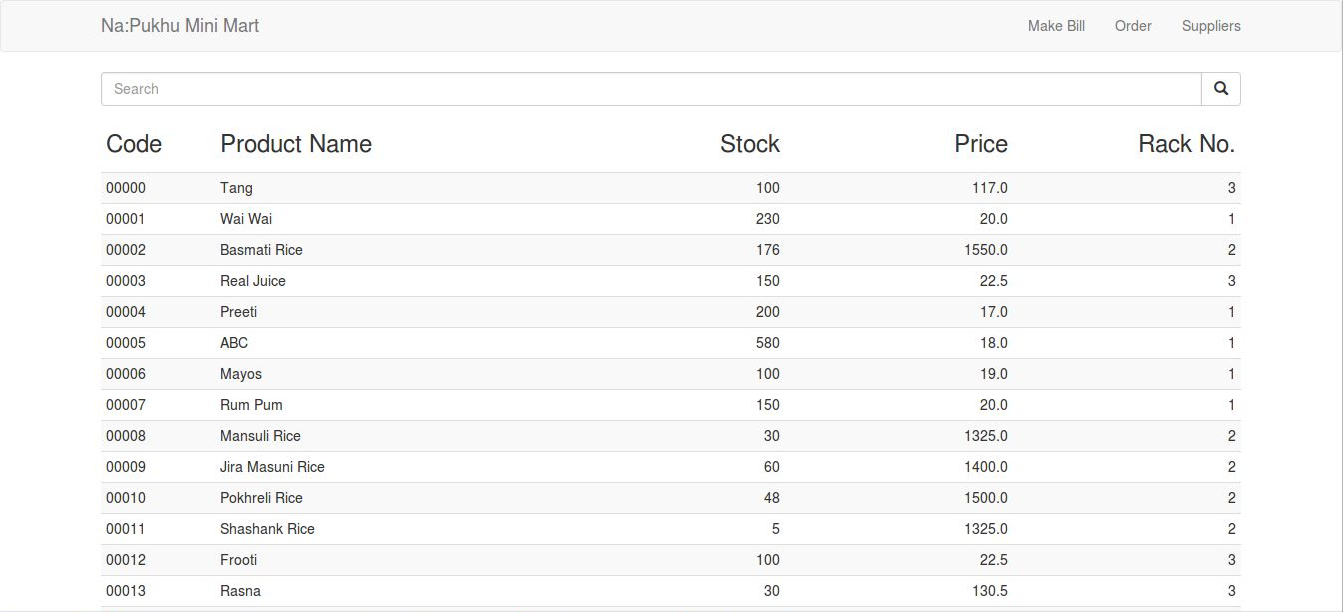
\includegraphics[width=6in]{fig/home}}
  \caption{Home page}\label{fig:home}
\end{figure}

\subsection{Make-Bill Page}

This page is used in order to prepare the bill for the products
bought by the customer. A staff simply enters the product code and quantity in
the designated areas and the product gets added into the bill. Once all the
products are added, the staff commits and the bill gets stored into the
database. There is also a reset button available for resetting the whole bill.

\begin{figure}[h!]\centering
  \fbox{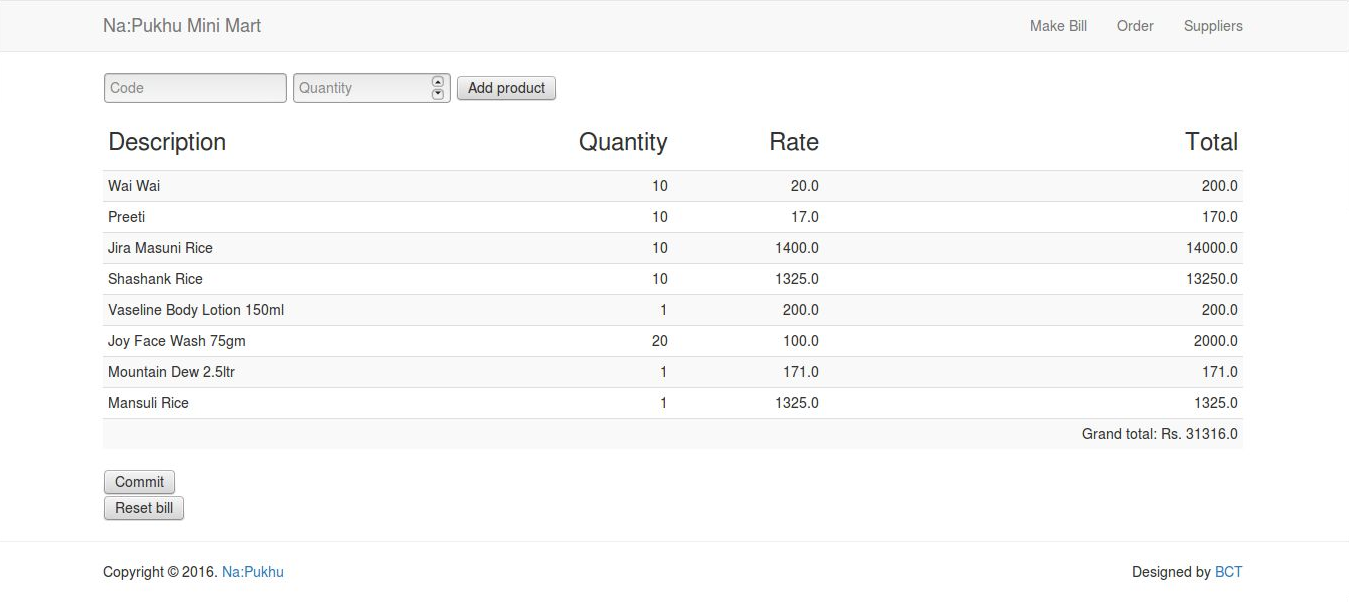
\includegraphics[width=6in]{fig/bill}}
  \caption{Make-bill page}\label{fig:bill}
\end{figure}

\subsection{Order Page}

This page is used to record the orders given to the product supplier as well as
the delivery made by the supplier. The page shows a list of recent orders. The
order contains the id, product name, quantity ordered, ordered date and status.
Once the order is recorded, it gets displayed in the list of orders and its
status is ``pending'' by default. After the delivery is made by the supplier, the
delivery detail is entered and thus the status of the pending order changes to
``delivered''.

\begin{figure}[h!]\centering
  \fbox{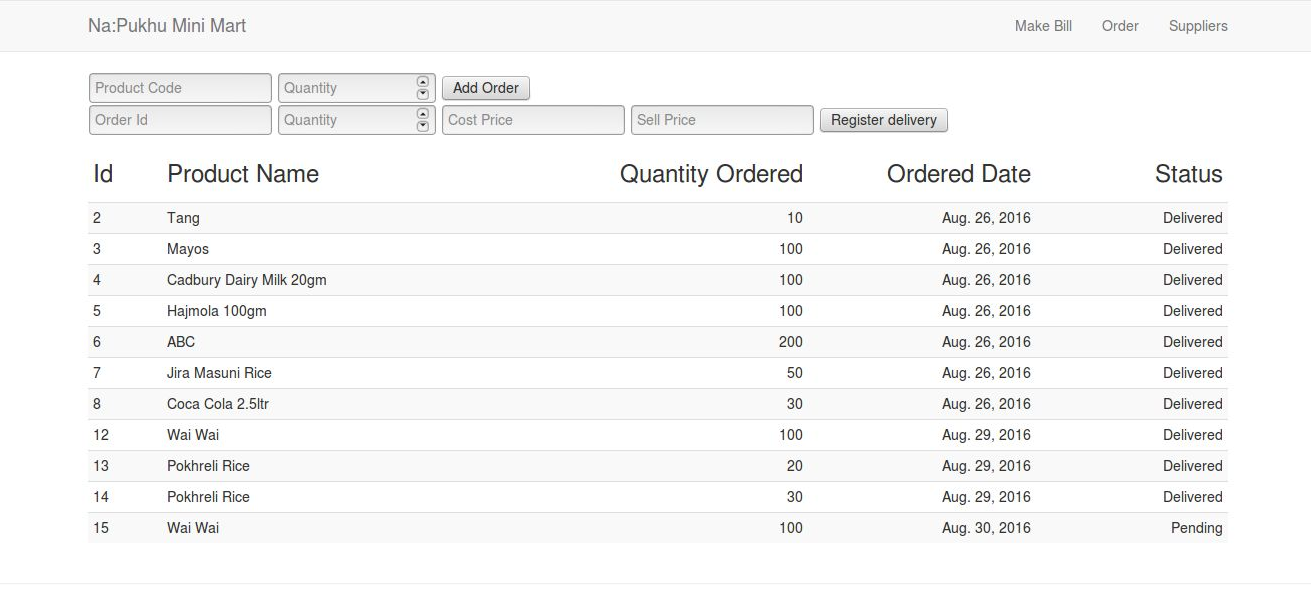
\includegraphics[width=6in]{fig/order}}
  \caption{Order page}\label{fig:order}
\end{figure}

\subsection{Supplier Page}

This page displays the list of suppliers that are associated with the
department store. It displays the name, address, contact number of the
supplier.

\begin{figure}[h!]\centering
  \fbox{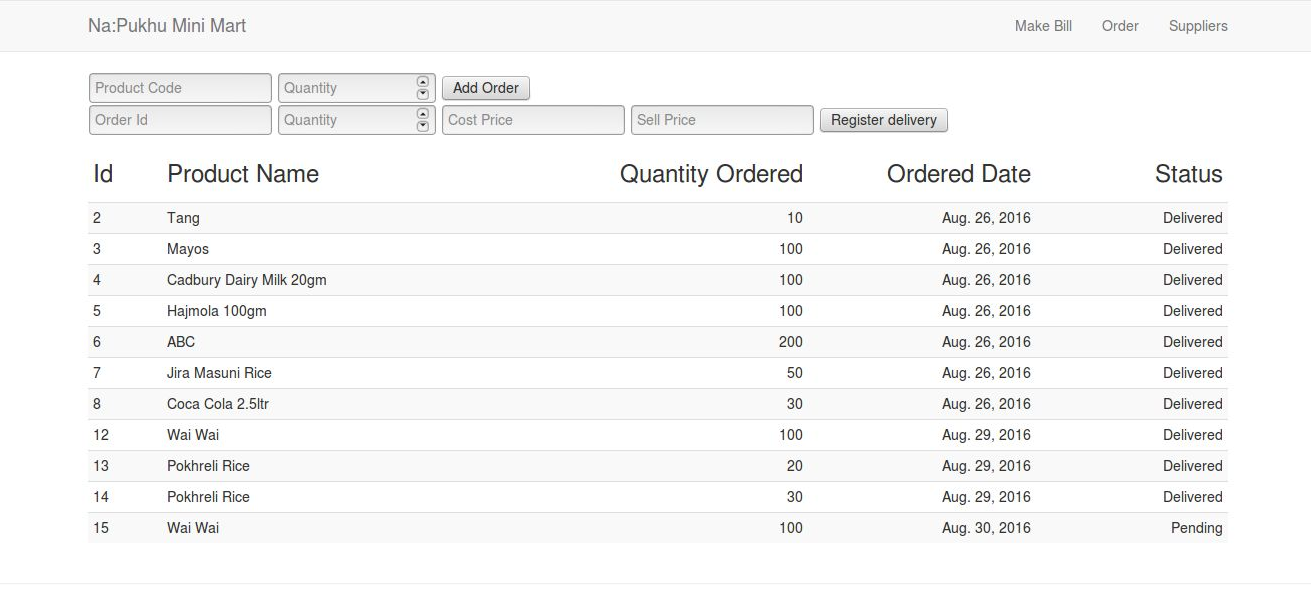
\includegraphics[width=6in]{fig/order}}
  \caption{Order page}\label{fig:order}
\end{figure}

\subsection{View-Bill Page}

This page is used to check out the past bills. The staff enters the bill number
and the system outputs the bill details. The detail consists of each and every
product bought, its rate, quantity, total and the grand total.

\begin{figure}[h!]\centering
  \fbox{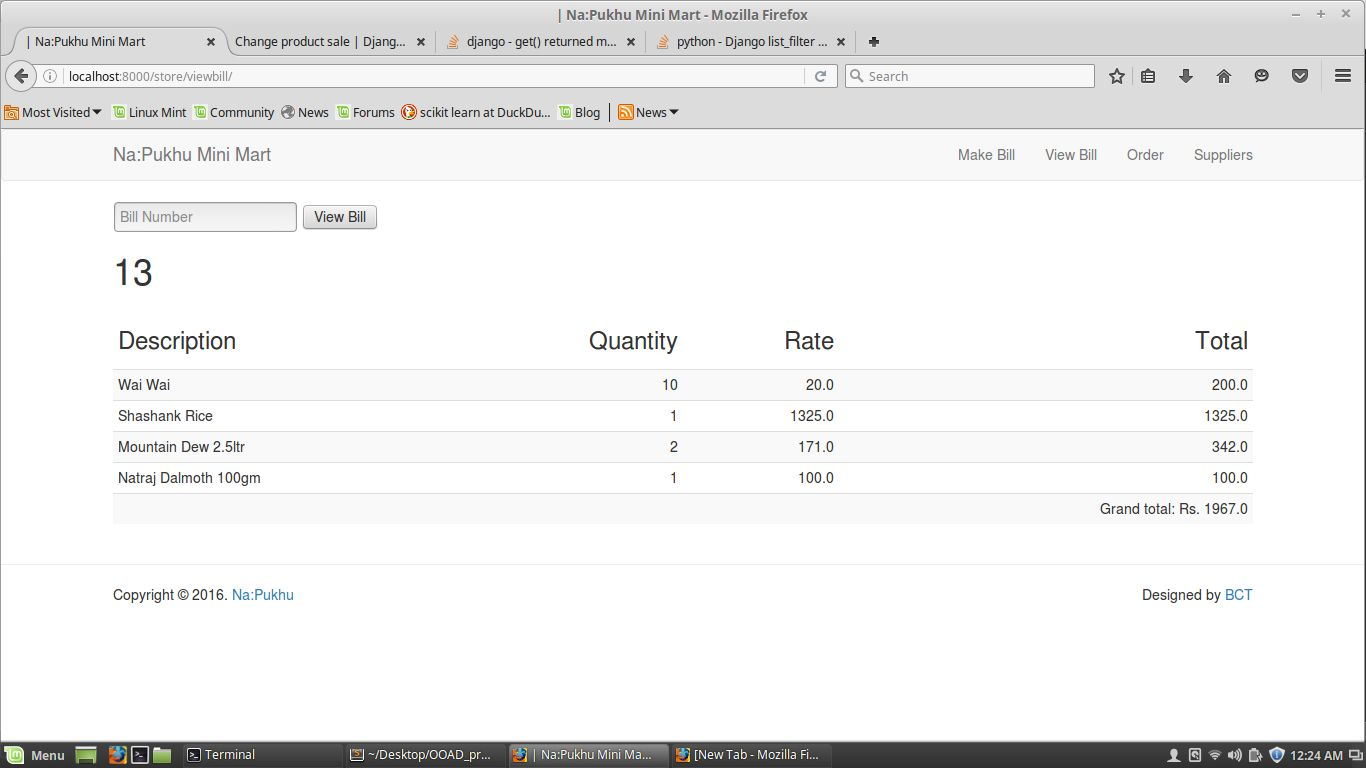
\includegraphics[width=6in]{fig/bill-info}}
  \caption{View-bill page}\label{fig:bill-info}
\end{figure}

We actually visited {\em Na: Pukhu Mini Mart} (located near Bhaktapur Mini Bus
Park, Itachhen) to know about managerial operations of the store and required
attributes for our database. This visit was helpful in understanding practical
approaches to manage a store.

Later section of this report contains Use Case and Class Diagram of the project
that gives overall overview of the system. \ldots
